\documentclass{article}

\usepackage{graphicx}
\usepackage{float}
\usepackage{amsmath}
\usepackage{geometry}
\usepackage{hyperref}
\usepackage{enumitem,amssymb}
\usepackage{todonotes}
\newlist{todolist}{itemize}{2}
\setlist[todolist]{label=$\square$}

\geometry{margin = 1in}

\title{\vspace{-2cm}Assignment 1 Geo5017}
\author{Job Segers (6597084), Timber Groeneveld (4213513), Akhil Veeranki (6305105)}
\date{\vspace{-4ex}}

\renewcommand{\thesubsubsection}{\thesection.\alph{subsubsection}}

\begin{document}

\maketitle

\section{Question 1}
\subsection{}
Perform data analysis to identify relevant features and relationships to define the exact model and the parameters to be fitted. 

\subsection{}
The set of parameters that minimizes the sum of squared errors. 

\section{Question 2}
\subsection{}
To plot the measured trajectory, we made Numpy arrays from the time stamps and positions of the drone, and then plotted both the positions and the trajectory between the positions using Matplotlib.


\begin{figure}[H]
    \centering
    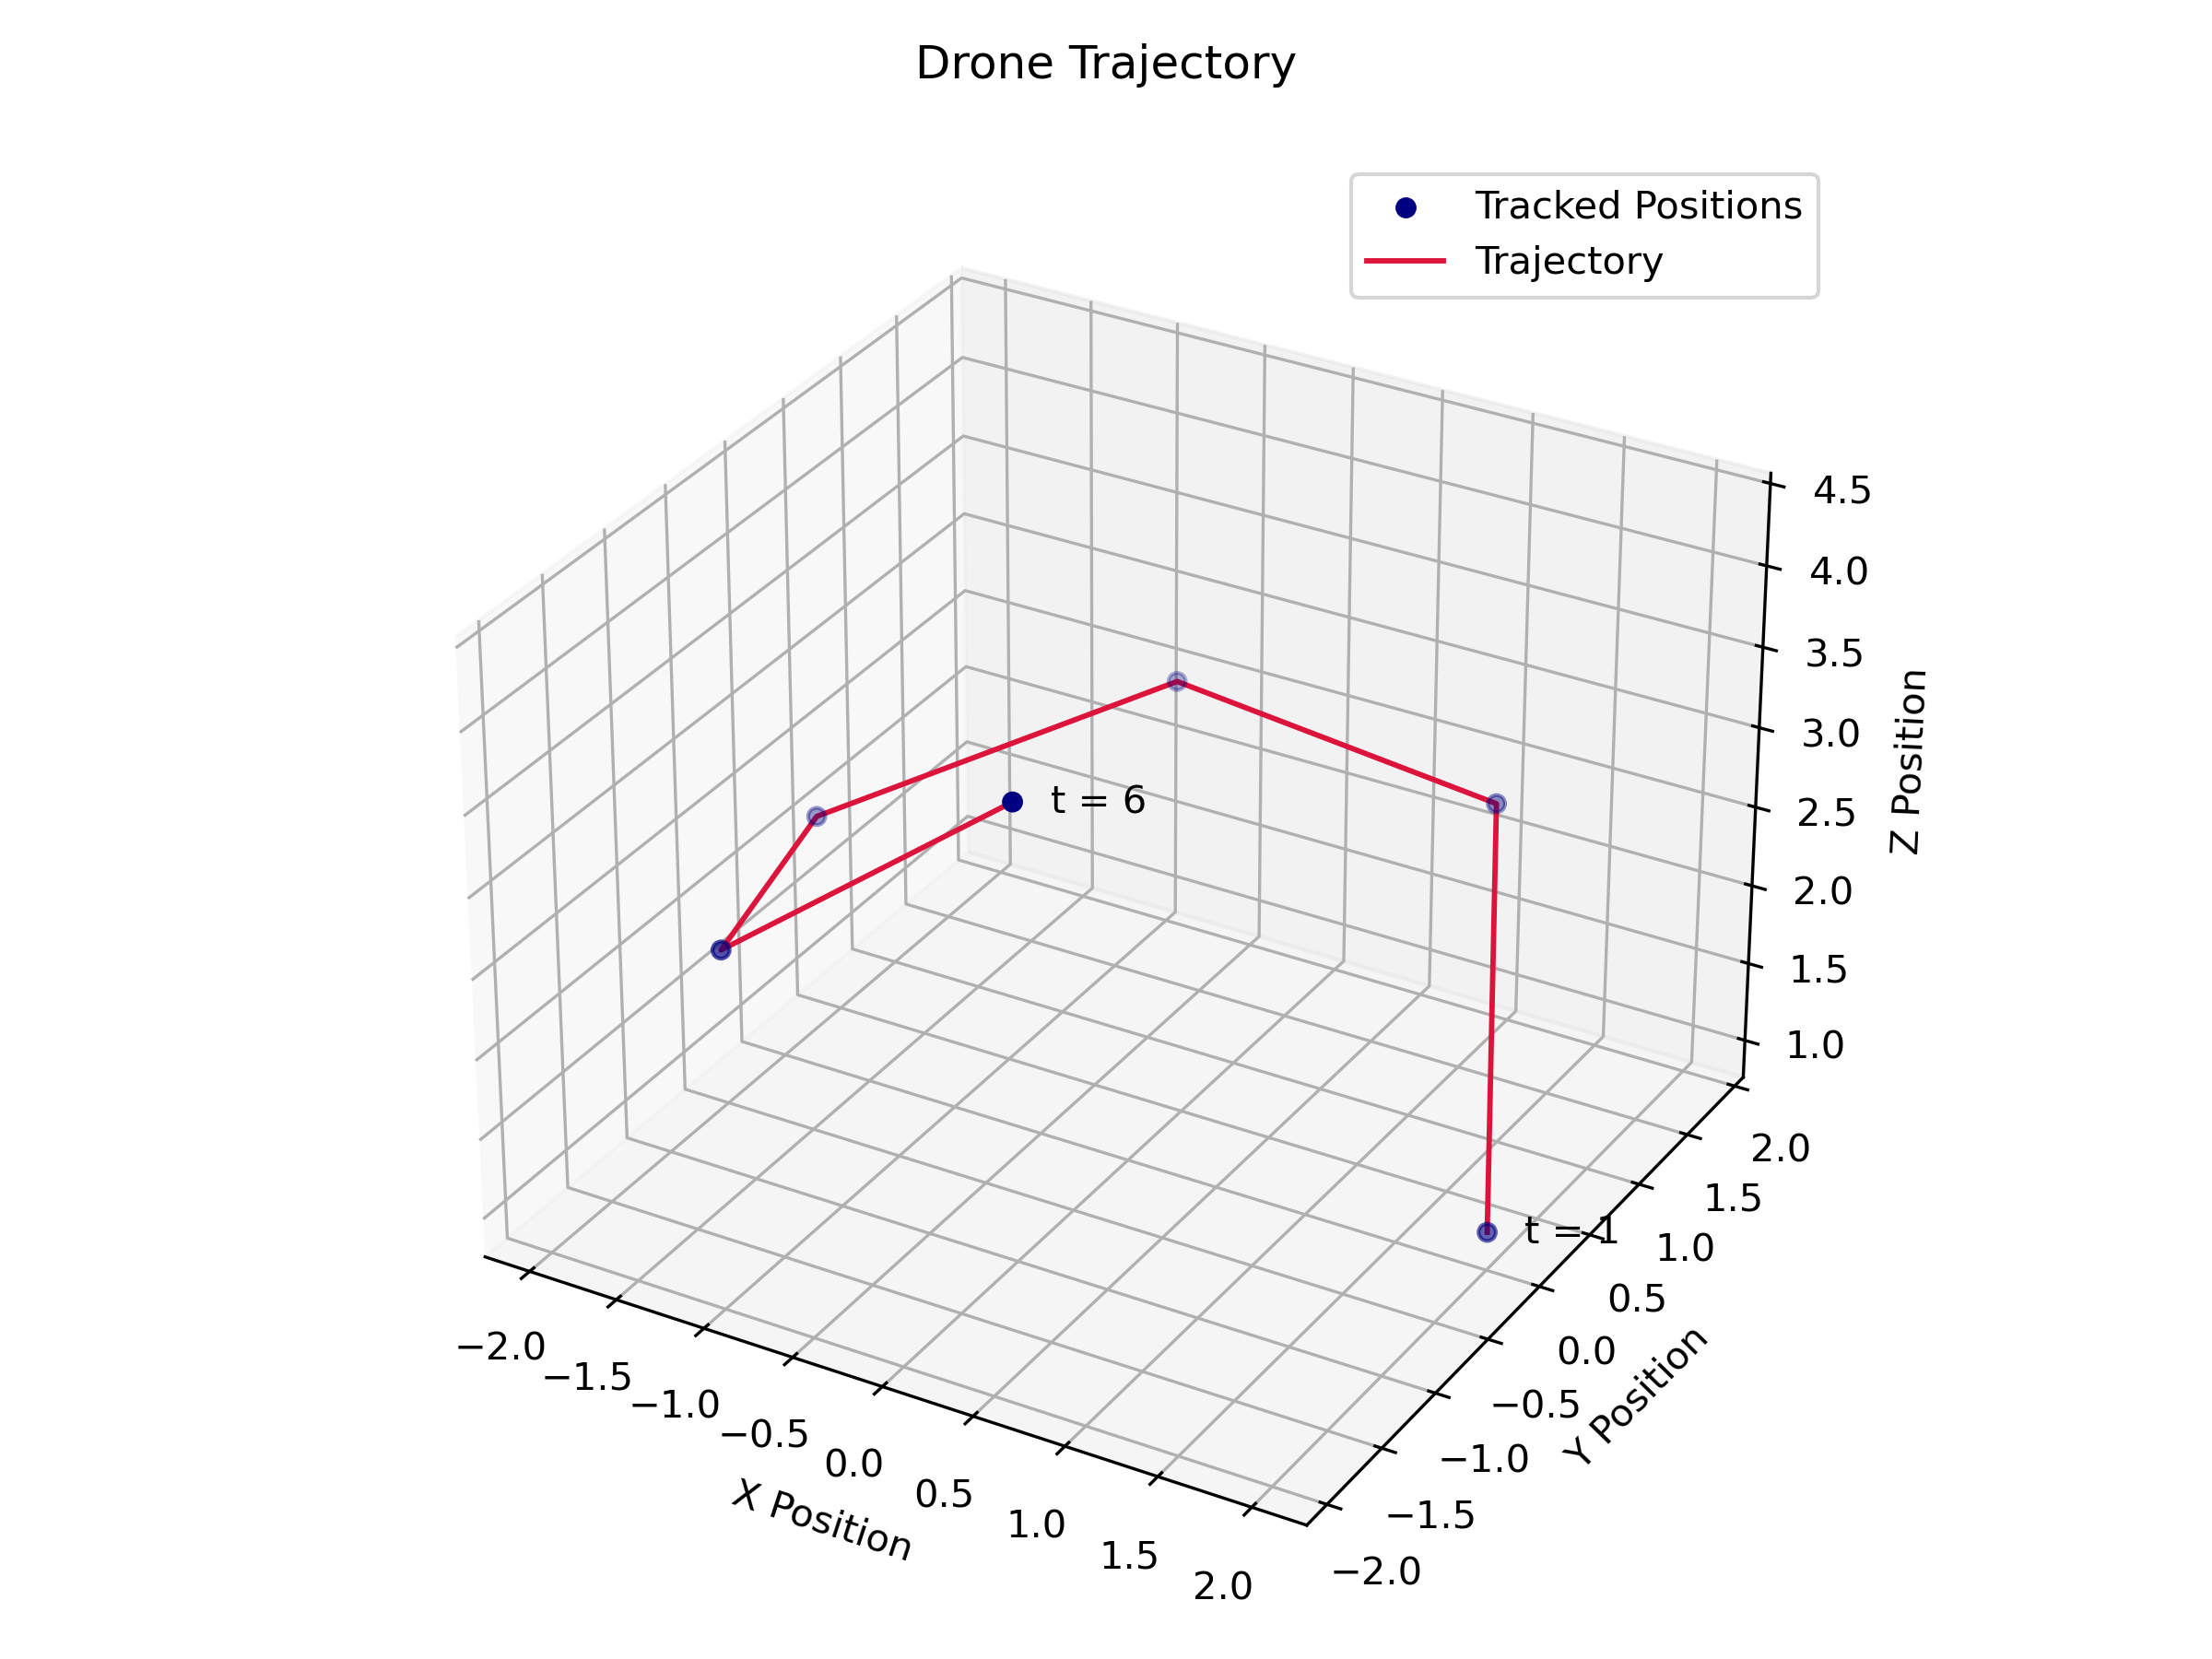
\includegraphics[width=0.75\textwidth]{Drone Trajectory.png}
    \caption{Tracked positions of the drone (blue) and the trajectory (red)}
    \label{fig:drone_tracking_connected_points}
\end{figure}


\subsection{}
\subsubsection{}
To make use of a gradient descent solve, we first need to define the model and the error function to be minimized. The model is as follows:
\begin{equation}
    \mathbf{x}_{pre} = \mathbf{v}t + \mathbf{x}_0
    \label{eq1}
\end{equation}
Where $\mathbf{x}_{pre}$,$\mathbf{v}$ and $\mathbf{x}_0$ are vectors with $x$,$y$ and $z$ components. As such this model has six unknowns: the components of the $\mathbf{v}$ and $\mathbf{x}_0$ vectors. For the error function we take the Euclidian distance between the actual point and the measured point. We thus want to minimize:
\begin{equation}
    E = \sum_i|\mathbf{x}_{i} -\mathbf{x}_{pre,i}|^2 = \sum_i|\mathbf{x}_i-(\mathbf{v}t_i+\mathbf{x_0})|^2
    \label{eq2}
\end{equation}
Calculating the gradient of this error function is simplified, since it can be separated into the sum of the $x$, $y$, and $z$ components. 
\begin{equation}
    E = \sum_i\sum_{k=(x,y,z)}(k_i - v_kt_i-k_0)^2
\end{equation}
This then yields the partial derivatives with regards to the components of the $\mathbf{v}$ and $\mathbf{x}_0$ as 
\begin{equation}
    \frac{\partial E}{\partial v_k} = -2\sum_i(k_i-v_kt_i-k_0)t_i
    \label{eq4}
\end{equation}
and
\begin{equation}
    \frac{\partial E}{\partial k} = -2\sum_i(k_i-v_kt_i-k_0)
    \label{eq5}
\end{equation}

Utilizing the calculated gradient we performed a gradient descent by taking steps in the direction of steepest descent, which is in the opposite direction of the gradient. A learning rate, a multiplier applied to the gradient to ensure manageable step sizes, of $10^{-3}$ was chosen to ensure that the algorithm converges without overshooting the minimum. The algorithm stops when the size of the parameter updates falls below the tolerance of $10^{-6}$, indicating that it closely approximated the minimum. The maximum number of iterations is set to $10^{5}$ as a safeguard. Further parameter tuning did not result in a lower SSE.

Using the provided positions and times, velocity is estimated through the gradient descent. The x,y and z components of the estimated velocity vector in the three dimensions are as follows:
\begin{equation}
\mathbf{v}^T \approx (-0.4417,\,-0.5903,\,0.4826)
\end{equation}

The remaining sum-of-squares error (SSE) of the constant velocity model is computed as in equation \ref{eq2}, using $\mathbf{v}$ and $\mathbf{x}_0$ estimated via the gradient descent solver. This yields:
\begin{equation}
E \approx 15.981 .
\end{equation}

\subsubsection{}
The constant acceleration model here is given as
\begin{equation}
    \mathbf{x}_{pre}=0.5\mathbf{a}t^2 + \mathbf{v}_0t+\mathbf{x_0}
\end{equation}
This model is similar to the previous one, but has three additional unknowns in the $x$,$y$ and $z$ components of the acceleration vector $\mathbf{a}$. The error function but includes an additional term, $-a_kt_i^2$, within the brackets. The gradient with respect to the initial velocity is similar to equations \ref{eq4} and \ref{eq5}. The gradient with respect to the acceleration vector components is
\begin{equation}
        \frac{\partial E}{\partial a_k} = -\sum_i(k_i-v_kt_i-k_0)t_i^2
\end{equation}
After fitting the constant acceleration model to the provided position and time samples, the residual error is computed as
\begin{equation}
E = \sum_i \left\| \mathbf{x}_i - \mathbf{x}_{pre,i} \right\|^2
  = \sum_i \left\| \mathbf{x}_i - \left(0.5\mathbf{a}t_i^2 + \mathbf{v}_0t_i + \mathbf{x}_0\right) \right\|^2
\end{equation}
Using the parameters estimated through our gradient descent solver, we obtain:
\begin{equation}
E \approx 4.942 .
\end{equation}
This error is lower than in the constant velocity case ($E \approx 15.981$) because the acceleration model is a second-order function of time and therefore has more degrees of freedom and more flexibility. Acceleration can represent change in velocity, whereas the constant velocity model can only represent a straight line of motion.
The SSE could be reduced further by using a higher-order polynomial model. However, with only six samples, increasing the number of parameters risks overfitting.

\subsubsection{}
Using the constant acceleration model and the gradient descent implementation, we trained a linear regression model. This was used to estimate the trajectory and to extrapolate to $t=7$. Together with the measured positions of the drone, this is plotted using Matplotlib. 

The estimated parameters obtained for the constant acceleration model are:
\[\mathbf{a} =\begin{bmatrix}0.8668 \\-0.6471 \\0.1096\end{bmatrix},
\quad\mathbf{v}_0 =\begin{bmatrix}-3.4756 \\1.6744 \\0.0990\end{bmatrix},
\quad\mathbf{r}_0 =\begin{bmatrix}5.5142 \\-0.8935 \\1.3107\end{bmatrix}.
\]

Using these parameters, the predicted position at $t=7$ is determined:
\[
\begin{aligned}
\mathbf{x}_{\mathrm{pre}}(7) &= (2.4229,\; -5.0257,\; 4.6888).
\end{aligned}
\]

\begin{figure}[H]
    \centering
    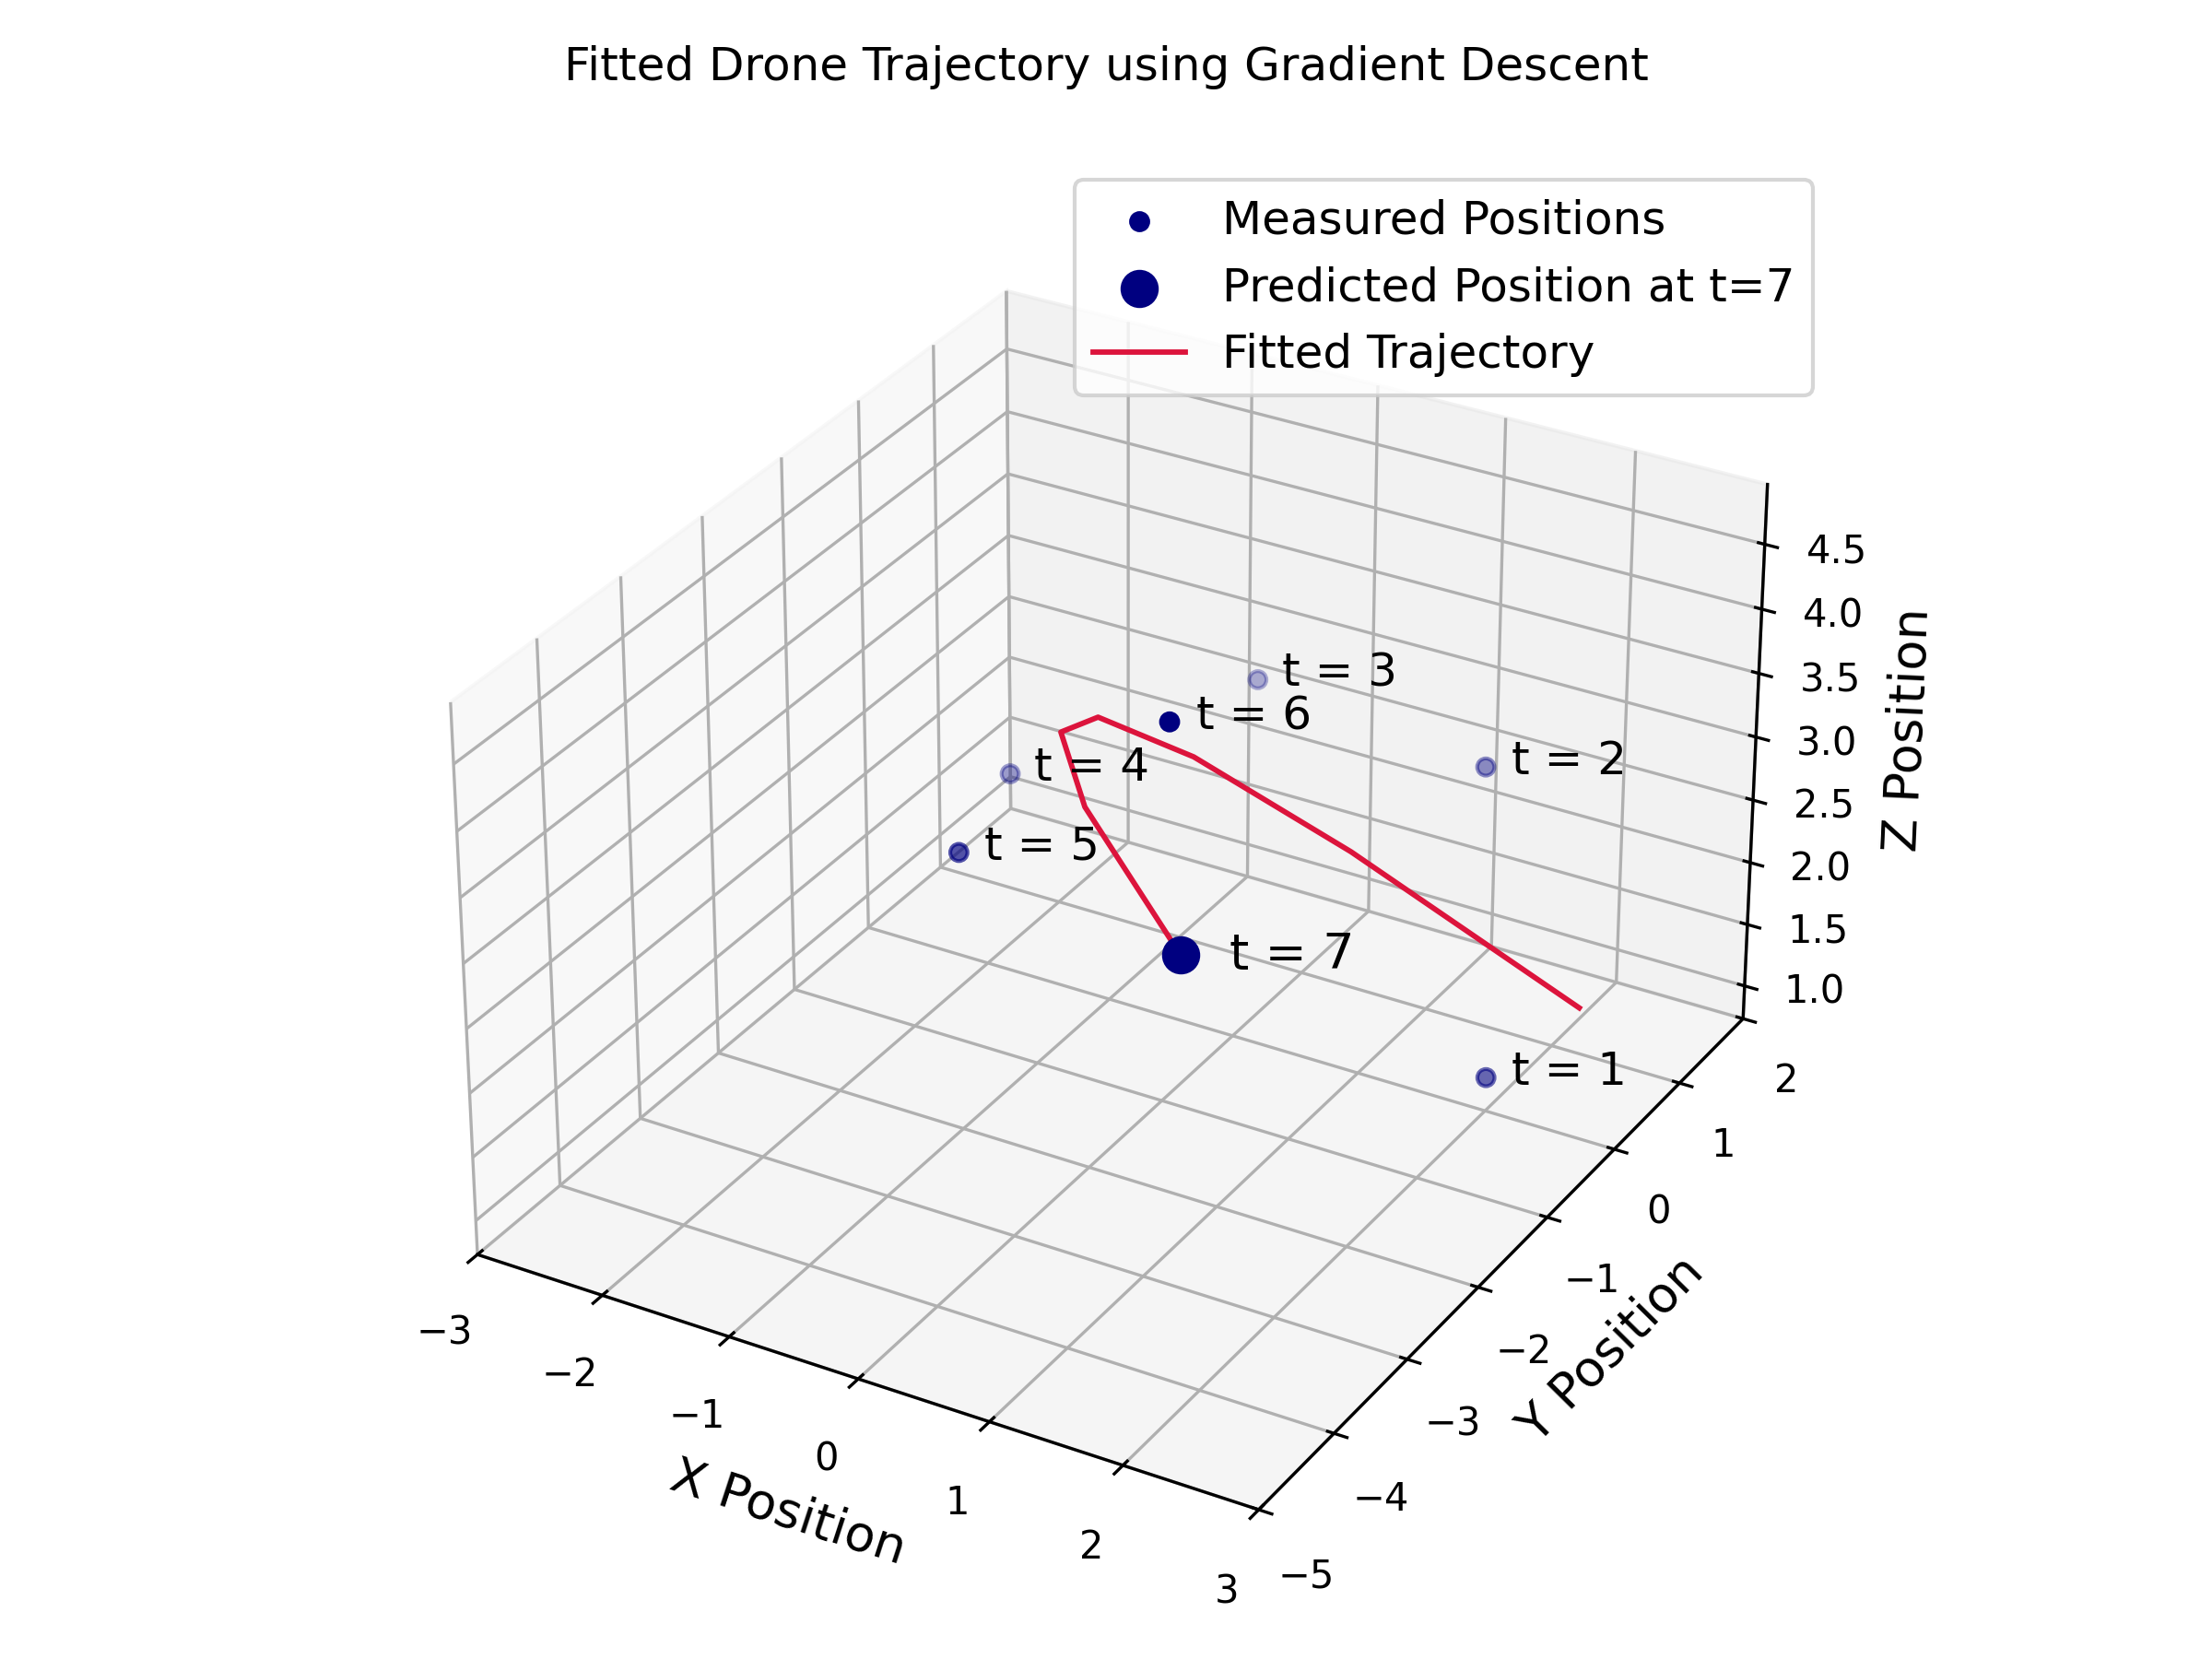
\includegraphics[width=0.99\textwidth]{Drone_Trajectory_With_Fit.png}
    \caption{Tracked positions of the drone (blue), estimated location at t=7 (blue, large) and the estimated trajectory (red).}
\label{fig:drone_trajectory_gradient_descent}
\end{figure}
The code used for this assignment can be accessed through \url{https://github.com/Jcsegertudelft/Geo5017ML_Assignment1}.

\section{Division of work}
\begin{table}[H]
    \centering
    \makebox[0pt]{
    \begin{tabular}{|c|c|c|}
    Job  & Timber & Akhil  \\
    \hline
    Set up Github and LaTeX template & Questions 1.1 and 1.2 answers & Write Python code for gradient descent \\
    Python code of models gradient & Python plot of the drone's trajectory & Code for residual error\\
    Math section 2.2.a and 2.2.b & 2.1 and 2.2.c extrapolation and plot & Answering numerical questions 2.2.a, 2.2.b\\
    ReadMe and small optimizations code &  & \\
    \end{tabular}}
    \label{tab:placeholder}
\end{table}

\end{document}